\chapter{Proprietà di correlazione}

\begin{figure}[h]
    \centering
    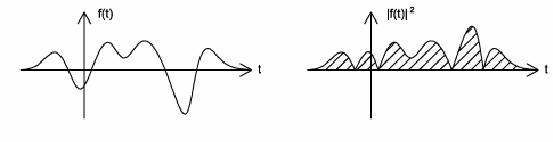
\includegraphics[scale = 1]{Esempio dell'energia di un segnale.jpg}
\end{figure}  

\newpage 

\section{Energia e potenza di un segnale nel tempo}

Per conoscere un segnale, non ci serve sapere tutto il segnale, bensì ci possono essere utili 
solo alcune sue caratteristiche. \newline 

Dato un segnale s(t) reale o complesso, si definisce energia 
totale E del segnale la seguente grandezza reale (se esiste): 

{
    \Large 
    \begin{equation}
        \begin{split}
            E 
            &=
            \lim_{\Delta t \rightarrow + \infty} 
            \int_{- \frac{\Delta t}{2}}^{\frac{\Delta t}{2}}
            s(t) \cdot s^{*}(t) dt 
            \\
            &=  \lim_{\Delta t \rightarrow + \infty} 
            \int_{- \frac{\Delta t}{2}}^{\frac{\Delta t}{2}}
            \abs{s(t)}^{2} dt \geq 0
        \end{split}
    \end{equation}
}

E può essere visto come l'energia totale dissipata da un resistore di 1 $\Omega$ quale ai suoi 
capi sia applicata la tensione s(t) [V]. \newline 

E può essere infinito, ma se $E>0$, allora si dice che s(t) è un segnale ad energia finita (o, sinteticamente, segnale di energia). \newline 

Un esempio di segnale di energia è l'impulso rettangolare con $E= \tau$ come il seguente: 

\begin{figure}[h]
    \centering
    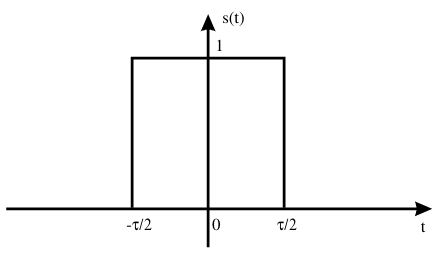
\includegraphics[scale = 1]{Impulso rettangolare con energia finita.PNG}
\end{figure}  

Se due segnali sono ortogonali, quindi: 

{
    \Large 
    \begin{equation}
        \int_{- \frac{\Delta t}{2}}^{+ \frac{\Delta t}{2}} s_1(t) \cdot s_2 ^{*} (t) dt = 0
    \end{equation}
}

allora, l'energia totale è la somma delle energie dei due segnali. \newline 

In formule: 

{
    \Large 
    \begin{equation}
        s(t) = s_1 (t) + s_2 (t)
    \end{equation}
}

{
    \Large 
    \begin{equation}
        \begin{split}
            E 
            &= 
            \lim_{\Delta t \rightarrow + \infty} 
            \int_{- \frac{\Delta t}{2}}^{\frac{\Delta t}{2}}
            [s_1 (t) + s_2 (t)] \cdot [s_1 ^{*} (t) + s_2 ^{*} (t)] dt 
            \\ 
            &= 
            \lim_{\Delta t \rightarrow + \infty} 
            \int_{- \frac{\Delta t}{2}}^{\frac{\Delta t}{2}}
            \abs{s_1 (t)} ^{2} dt 
            + 
            \int_{- \frac{\Delta t}{2}}^{\frac{\Delta t}{2}}
            \abs{s_2 (t)} ^{2} dt 
            + 
            2 \Re [\int_{- \frac{\Delta t}{2}}^{\frac{\Delta t}{2}}
            s_1 (t) \cdot s_2 ^{*} (t) dt] 
            \\
            &= E_1 + E_2 + 0 
            \\ 
            &= E_1 + E_2
        \end{split}
    \end{equation}
}

Dato un segnale s(t) reale o complesso, 
possiamo definire la potenza totale P del segnale la grandezza reale: 

{
    \Large 
    \begin{equation}
        \begin{split}
        P 
        &= 
        \lim_{\Delta t \rightarrow + \infty} 
        \frac{1}{\Delta t}
        \int_{- \frac{\Delta t}{2}}^{\frac{\Delta t}{2}} 
        s(t) \cdot s^{*} (t) dt 
        \\ 
        &= 
        \lim_{\Delta t \rightarrow + \infty} 
        \frac{1}{\Delta t}
        \int_{- \frac{\Delta t}{2}}^{\frac{\Delta t}{2}} 
        \abs{s(t)} ^{2} dt 
        \geq 0
        \end{split}
    \end{equation}
}

Se P risulta finito e maggiore di zero, il segnale si dice di potenza finita 
(o sinteticamente, segnale di potenza). \newline 

Un segnale di potenza ha sempre energia infinita, mentre non sempre è vero il viceversa. \newline 

D'altro canto, un segnale ad energia finita ha potenza nulla. \newline 

Quindi, la potenza e l'energia sono due caratteristiche diverse di un segnale. \newline 

\newpage 

\section{Energia e potenza di un segnale in frequenza}

\subsection{Teorema di Parseval} 

Possiamo esprimere l'energia e la potenza di un segnale s(t) anche utilizzando 
il dominio della frequenza: 

{
    \Large 
    \begin{equation}
        \begin{split}
            E 
            &= 
            \int_{- \infty}^{+\infty} 
            \abs{s(t)} ^{2} dt 
            \\
            &= 
            \frac{1}{2 \pi} 
            \int_{- \infty}^{+\infty} 
            \abs{S(\omega)} ^{2} dt 
        \end{split}
    \end{equation}
}

Se s(t) è un segnale periodico, per definizione, possiamo integrare nel periodo, quindi: 

{
    \Large 
    \begin{equation}
     \begin{split}
        E 
        &= 
        \int_{- \frac{T}{2}}^{\frac{T}{2}} 
        \abs{s(t)} ^{2} dt 
        \\ 
        &= \sum_{\kappa = - \infty}^{+\infty}
        \abs{c_\kappa} ^{2} 
     \end{split}   
    \end{equation}
            
}

Considerando la relazione tra pulsazione e frequenza: 

{
    \Large 
    \begin{equation}
        \omega = 2 \pi f
    \end{equation}
}

possiamo esprimere E in funzione di f: 

{
    \Large 
    \begin{equation}
        E = \int_{- \infty}^{+ \infty} 
        \abs{S(f)} ^{2} df
    \end{equation}
}

Questa ultima espressione prende il nome di densità spettrale, misurata in Hz. \newline 

\newpage 

\subsection{Dimostrazione del Teorema di Parseval} 

Consideriamo due segnali $s_1 (t)$ e $s_2 (t)$ e consideriamo le loro trasformate 
$S_1 (\omega)$ e $S_2 (\omega)$ : 

{
    \Large 
    \begin{equation}
        \begin{split}
            F[s_1(t) \cdot s_2(t)]
            &=
            \frac{1}{2 \pi} 
            S_1 (\omega) \otimes S_2 (\omega) 
            \\ 
            &= 
            \frac{1}{2 \pi}
            \int_{-\infty}^{+ \infty}
            S_1 (\Omega) \cdot S_2 (\omega - \Omega)  
            d\Omega
        \end{split}
    \end{equation}
}

dove $\otimes$ indica l'espressione di convoluzione e $\omega$ è usato come parametro. \newline 

Dunque: 

{
    \Large 
    \begin{equation}
        \int_{- \infty}^{+ \infty} 
        s_1 (t) s_2 (t) e^{-\jmath \omega t} dt 
        = 
        \frac{1}{2 \pi} 
        \int_{- \infty}^{+ \infty}
        S_1 (\Omega) S_2 (\omega - \Omega) d\Omega
    \end{equation}
}

Ponendo: 

{
    \Large 
    \begin{equation}
        \omega = 0
    \end{equation}
}

l'integrale in frequenza sarà: 

{
    \Large 
    \begin{equation}
        \int_{- \infty}^{+ \infty} 
        s_1 (t) s_2 (t) e^{-\jmath \omega t} dt 
        = 
        \frac{1}{2 \pi} 
        \int_{- \infty}^{+ \infty}       
        S_1 (\Omega) S_2 (- \Omega) d\Omega
    \end{equation}
}

Ponendo: 

{
    \Large 
    \begin{equation}
        s_1 (t) = s_2 ^{*}(t) = s(t)
        \leftrightarrow 
        S_1 (\omega) = S_2 ^{*} (\omega) = S(\omega)
    \end{equation}
}

l'integrale si riduce in: 

{
    \Large 
    \begin{equation}
            \int_{- \infty}^{+\infty} 
            \abs{s(t)} ^{2} dt 
            \\
            = 
            \frac{1}{2 \pi} 
            \int_{- \infty}^{+\infty} 
            \abs{S(\omega)} ^{2} dt 
    \end{equation}
} 

\newpage 

\subsection{Definizione di potenza in frequenza}

Definiamo un segnale troncato $s_\Delta (t)$: 

{
    \Large 
    \begin{equation}
        s_\Delta (t) 
        = 
        \begin{cases}
            s(t) 
            \text{ in } 
            \abs{t} \leq \frac{\Delta t}{2} 
            \\ 
            0 
            \text{ in } 
            \abs{t} \ge \frac{\Delta t}{2}
        \end{cases} 
    \end{equation}
}

Dal punto di vista grafico, andremo a considerare la porzione di questo segnale di esempio: 

\begin{figure}[h]
    \centering
    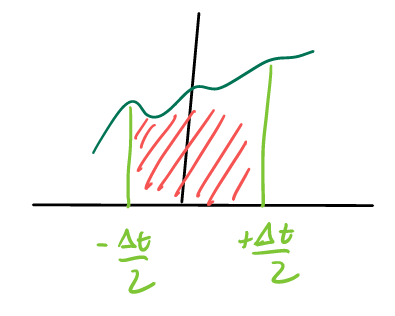
\includegraphics[scale = 0.8]{Calcolo di un'energia di un segnale esempio.PNG}
\end{figure}  


L'energia di questo segnale sarà: 

{
    \Large 
    \begin{equation}
        \begin{split}
            E_\Delta 
            &= 
            \int_{- \frac{\Delta t}{2}}^{\frac{\Delta t}{2}}
            \abs{s(t)} ^{2} dt 
            \\ 
            &= \frac{1}{2 \pi} 
            \int_{- \frac{\Delta t}{2}}^{\frac{\Delta t}{2}}
            \abs{S_\Delta (\omega)} ^{2} d\omega 
        \end{split}
    \end{equation}
}

in cui $S_\Delta (\omega)$ è la trasformata di Forurier di $s_\Delta (t)$. \newline 

Ora possiamo definire la potenza di un segnale anche in frequenza: 

{
    \Large 
    \begin{equation}
        \begin{split}
            P 
            &= 
            \lim_{\Delta t \rightarrow \infty}
            \frac{E_\Delta}{\Delta t} 
            \\ 
            &= 
            \lim_{\Delta t \rightarrow \infty}
            \frac{1}{\Delta t} 
            [\frac{1}{2 \pi} \int_{- \infty}^{+ \infty} 
            \abs{S_\Delta (\omega)}^{2} d\omega]
            \\ 
            &= 
            \frac{1}{2 \pi} 
            \int_{- \infty}^{+ \infty}
            \lim_{\Delta t \rightarrow \infty} 
            \frac{\abs{S_\Delta (\omega)}^{2}}{\Delta t} d\omega
        \end{split}
    \end{equation}
}

Quindi possiamo definire: 

{
    \Large 
    \begin{equation}
        p(\omega) 
        = 
        \lim_{\Delta t \rightarrow \infty} 
        \frac{\abs{S_\Delta (\omega)}^{2}}{\Delta t} d\omega
    \end{equation}
}

$p(\omega)$ prende il nome di densità spettrale di potenza. \newline 

P, usando la densità spettrale di potenza, sarà definita come: 

{
    \Large 
    \begin{equation}
        P 
        = 
        \frac{1}{2 \pi}
        \int_{-\infty}^{+ \infty}
        p(\omega) d\omega 
    \end{equation}
}

Utilizzando la frequenza, in particolare lo spettro di potenza, possiamo definire la potenza come: 

{
    \Large 
    \begin{equation}
        P = \int_{- \infty}^{\infty}
        p(f) df 
    \end{equation}
}

\newpage

\section{Relazione tra energia, potenza, spettri e autocorrelazione} 

Definiamo l'autocorrelazione di un segnale di energia s(t) come: 

{
    \Large
    \begin{equation}
        R_s = \int_{- \infty}^{+ \infty}
        s^{*} (t) s(t + \tau) dt 
    \end{equation}
} 

Se $\tau = 0$: 

{
    \Large 
    \begin{equation}
        R_s (\tau = 0) = E
    \end{equation}
}

Se s(t) è un segnale reale, possiamo definire l'autocorrelazione del segnale come: 

{
    \Large 
    \begin{equation}
        R_s = s(t) \otimes s(-t)
    \end{equation}
}

Quindi, dal punto di vista computazione è come la convoluzione tra due segnali, 
ma in questo caso, non viene fatta nessuna inversione dell'asse temporale, bensì la funzione 
viene solo traslata per $\tau$. \newline 

Se il segnale s(t) è reale pari, $R_s (\tau)$ coincide esattamente con la convoluzione del segnale con se stesso. \newline 

Applicando la proprietà della convoluzione, possiamo scrivere che: 

{
    \Large 
    \begin{equation}
        F[R_s (t)] = \abs{S(\omega)} ^{2}
    \end{equation}
}

Dunque, la trasformata di Forurier della funzione autocorrelazione, coincide con lo spettro di energia del segnale. \newline 

Per segnali di potenza, la definizione di autocorrelazione deve essere modificata come: 

{
    \Large 
    \begin{equation}
        R_s (\tau) = \lim_{\Delta t \rightarrow \infty} 
        \frac{1}{\Delta t} 
        \int_{- \frac{\Delta t}{2}}^{\frac{\Delta t}{2}}
        s^{*} (t) s(t + \tau) dt
    \end{equation}
}

Se $\tau = 0$: 

{
    \Large 
    \begin{equation}
        R_s (\tau = 0) = P
    \end{equation}
}

Come l'autocorrelazione, facendo la trasformata di Forurier di $R_s (\tau)$ 
di un segnale di potenza, avremo che: 

{
    \Large 
    \begin{equation}
        F[R_s (\tau)] = p(\omega)
    \end{equation}
}

Nel caso di segnali periodici, avremo che: 

{
    \Large 
    \begin{equation}
        \begin{split}
            R_s (\tau) 
            &=
            \frac{1}{T} 
            \int_{- \frac{T}{2}}^{\frac{T}{2}} 
            s^{*} (t) s(t + \tau) dt 
            \\ 
            &= \frac{1}{T} 
            \int_{- \frac{T}{2}}^{\frac{T}{2}}
            \sum_{\kappa = - \infty}^{+\infty}
            c_\kappa ^{*} \frac{1}{\sqrt{T}} 
            e^{- \jmath \kappa \omega_0 t}
            \sum_{h = - \infty}^{+\infty}
            c_h \frac{1}{\sqrt{T}} 
            e^{\jmath h \omega_0 (t + \tau)} 
            dt 
            \\ 
            &= 
            \frac{1}{T^{2}} 
            \sum_{\kappa = - \infty}^{+\infty} 
            \sum_{h = - \infty}^{+\infty} 
            c_\kappa ^{*} c_h 
            e^{-\jmath h \omega_0 \tau}
            \int_{-\frac{T}{2}}^{\frac{T}{2}} 
            e^{-\jmath \kappa \omega_0 t} 
            e^{\jmath h \omega_0 t} 
            dt
        \end{split}
    \end{equation}
} 

Grazie alla proprietà di ortogonalità tra le due funzioni sinusoidali, 
visto anche nella sezione "2.3 Ortogonalità tra due segnali", abbiamo che: 

{
    \Large 
    \begin{equation}
        \int_{-\frac{T}{2}}^{\frac{T}{2}}
        e^{-\jmath \kappa \omega_0 t}
        e^{\jmath h \omega_0 t}
        dt 
        = 
        \begin{cases}
                T \text{ se } \kappa = h \\ 
                0 \text{ se } \kappa \neq  h 
        \end{cases}
    \end{equation}
}

Sostituendo questa proprietà di ortogonalità tra le due funzioni sinusoidali, 
avremo che: 

{
    \Large 
    \begin{equation}
        \begin{split}
            R_s (\tau)
            &= 
            \frac{1}{T} 
            \int_{- \frac{T}{2}}^{+\frac{T}{2}} 
            s^{*} (t) s(t + \tau) dt 
            \\
            &= 
            \frac{1}{T} 
            \sum_{\kappa = \infty}^{+\infty} 
            \abs{c_\kappa}^{2} 
            e^{\jmath \kappa \omega_0 \tau}
        \end{split}
    \end{equation}
}

Considerando la trasformata di Forurier di $R_s(\tau)$, abbiamo che: 

{
    \Large 
    \begin{equation}
        F[R_s (\tau)] 
        = 
        p(\omega) 
        = 
        \frac{2 \pi}{T} 
        \sum_{\kappa = - \infty}^{+\infty}
        \abs{c_\kappa} ^{2} 
        \delta (\omega - \kappa \omega_0)
    \end{equation}
} 

dove $\delta (\omega)$ è l'impulso matematico, o Delta di Dirac. \newline 

Ponendo, $\Delta t = NT$ dove N è un numero intero e T è il periodo del segnale, abbiamo che la potenza 
del segnale periodico è: 

{
    \Large 
    \begin{equation}
        \begin{split}
            P 
            &= 
            \lim_{N \rightarrow +\infty} 
            \frac{1}{NT} 
            \int_{-\frac{NT}{2}}^{\frac{NT}{2}} 
            \abs{s(t)}^{2} 
            dt 
            \\ 
            &=
            \lim_{N \rightarrow +\infty} 
            \frac{N}{NT} 
            \int_{-\frac{T}{2}}^{\frac{T}{2}} 
            \abs{s(t)}^{2} 
            dt
            \\
            &=  
            \frac{1}{T} 
            \int_{-\frac{T}{2}}^{\frac{T}{2}} 
            \abs{s(t)}^{2} 
            dt
        \end{split}
    \end{equation}
}

Sapendo inoltre che, per un segnale periodico: 

{
    \Large 
    \begin{equation}
        \int_{-\frac{T}{2}}^{\frac{T}{2}} 
            \abs{s(t)}^{2} 
            dt 
            =
            \sum_{\kappa = - \infty}^{+ \infty} 
            \abs{c_\kappa}^{2}
    \end{equation}
} 

e che per definizone l'integrale della Delta di Dirac da $[- \infty,  + \infty]$ è uguale a uno, 
possiamo esprimere la potenza di un segnale periodico come: 

{
    \Large 
    \begin{equation}
        P = \frac{\sum_{\kappa = - \infty}^{+ \infty} 
        \abs{c_\kappa}^{2}}{T}
    \end{equation}
}

Invece, per due segnali $s_1 (t)$ e $s_2 (t)$, possiamo definire la correlazione mutua, 
che possiamo vederla come la generalizzazione dell'autocorrelazione, come: 

{
    \Large 
    \begin{equation}
        R_{12} 
        = 
        \int_{- \infty}^{+ \infty}
        s_1 (t + \tau) 
        s_2 ^{*} (t) 
        dt 
    \end{equation}
}

Con la stessa procedura della correlazione, abbiamo che: 
{
    \Large 
    \begin{equation}
        F [R_{12}] 
        = 
        S_{12} (\omega) 
        = 
        S_1 (\omega) 
        S_2 ^{*} (\omega)
    \end{equation}
} 

dove, $S_{12} (\omega)$ prende il nome di spettro di energia mutua di due segnali. \newline 

\newpage 
.
\newpage 
.
\newpage 
